\documentclass[a4paper,10pt]{article}
\usepackage[utf8x]{inputenc}

\usepackage[left=2.5cm,right=2.5cm,top=2cm,bottom=2cm]{geometry}
\usepackage{amsmath,amsfonts,amssymb}
\usepackage{graphicx}
\usepackage[colorlinks=true,linkcolor=blue,urlcolor=blue,citecolor=blue]{hyperref}
\usepackage{color}
\usepackage{listings}

%opening
\title{Skippy Device Server}
\author{Sergi Blanch-Torn\'e\\\small{Controls Software Engineer - Alba Synchrotron}\\{\tt \small{sblanch@cells.es}}}

\newcommand{\todo}[1]{\texttt{\color{red}TODO:} ``\emph{#1}''}
\newcommand{\fixme}[1]{\texttt{\color{red}FIXME:} ``\emph{#1}''}
\newcommand{\ok}[1]{``#1'' [\texttt{\color{green}OK}]}

\begin{document}

\maketitle

\begin{abstract}
Following the \href{https://en.wikipedia.org/wiki/Standard_Commands_for_Programmable_Instruments}{wikipedia}'s definition:  the SCPI ``\emph{defines a standard for syntax and commands to use in controlling programmable test and measurement devices}''. Many scientific instrumentation uses this schema for the configuration and operation of the instrument of its purpose.

Alba has used an specific Device Server, under the name \emph{PyVisaInstrWrapper}, to communicate with instruments like scopes, radio frequency generators, arbitrary signal generators and spectrum analyser. This device was an extension from the original PyScope, becoming it one of the internal device classes. Many improvements has been introduced to this Device Server, but nowadays it is showing the limit of this design. A complete refactoring is needed.
\end{abstract}

\section{Design}

The main restriction that the PyVisaInstrWrapper shows is the dependency on the PyVisa subdevice to manage the communications with the instrument. Also the growing number of query commands to the instrument has reach the limit of the basic design.

\subsection{Machine state}

\begin{figure}[h]
    \centering{
         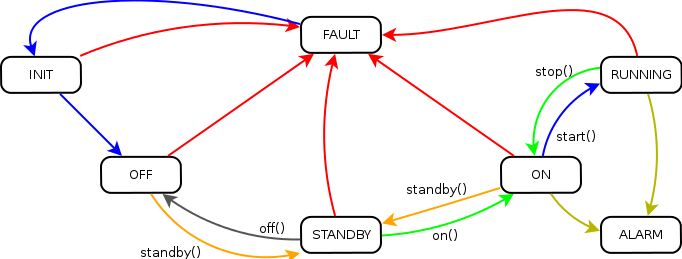
\includegraphics[width=0.75\textwidth]{StateMachine.png}
         \caption{State machine diagram of the Device in the Skippy Device Server} \label{fig:stateMachine}
    }
\end{figure}

\todo{explain the figure \ref{fig:stateMachine}}

\subsection{Device Properties}

\begin{itemize}
    \item Instrument: mandatory property to configure the instrument that will be introduced to the distributed system via the device.
    \begin{itemize}
        \item If the content string is a host name, use sockets to communicate with the instrument
        \item If the content string is a device name and the class of it is a PyVisa, use it as the bridge to the instrument.
        \item else, decay to fault state with the appropriate status message
    \end{itemize}
    \item Port: optional property to specify a port, in the socket communication, when it should be different than the default 5025.
    \item NumChannels: optional property to define, in case the instrument has channels, the number of them available.
    \item NumFunctions: optional property to define, in case the instrument has functions, the number of them available.
\end{itemize}

\subsection{Device Commands}

\begin{itemize}
    \item IDN(): Request identification to the instrument.
    \item Off(): Release the communication with the instrument.
    \item On(): Stablish communication with the instrument.
    \item Start(): Start an active monitoring.
    \item Stop(): Stop the active monitoring.
    \item OpenCh(): In case the instrument has channels open the numbered in the argin.
    \item CloseCh(): In case the instrument has channels close the numbered in the argin.
    \item OpenFn(): In case the instrument has functions open the numbered in the argin.
    \item CloseFn(): In case the instrument has functions close the numbered in the argin.
\end{itemize}

\subsection{Device Attributes}

\begin{itemize}
    \item idn: read attribute with the identification of the instrument linked.
\end{itemize}

Other attributes can be built using a \href{http://en.wikipedia.org/wiki/Builder_pattern}{Builder pattern}. In fact, when the device starts and the instrument is identified, with the information provided in this identification, the device can find how to build the instructions set.

An example of an attribute definition:

\begin{lstlisting}[language=python,basicstyle=\footnotesize]
Attribute('State',
          {'type':PyTango.CmdArgType.DevBoolean,
           'dim':[0],
           'readCmd':lambda ch,num:":%s%d:DISPlay?"%(ch,num),
           'writeCmd':lambda ch,num:(lambda value:":%s%d:DISPlay %s"%(ch,num,value)),
           'channels':True,
           'functions':True,
         })
\end{lstlisting}

This example, in a oscilloscope with 4 channels and 4 functions, will setup 8 {\tt READ\_WRITE} boolean attributes, called with the pattern: {\tt State\{Ch,Fn\}[1..4]}. Point to comment is the {\tt readCmd} and the {\tt writeCmd} and the use of {\tt lambda}s. In the \emph{read} case, and because this is an attribute description to build more than one, the {\tt lambda} function is set to build the final command for each of the channels and functions. A bit more complicated is the \emph{write} case, where there are two nested {\tt lambda}s, one used in the attribute build and the other used when write the attribute because is when the value is known.

Another example of an attribute definition:

\begin{lstlisting}[language=python,basicstyle=\footnotesize]
Attribute('Frequency',
          {'type':PyTango.CmdArgType.DevDouble,
           'dim':[0],
           'readCmd':":FREQ?",
           'writeCmd':lambda value:":FREQ %s"%(str(value)),
           'rampeable':True,
         })
\end{lstlisting}

That example, in a RF generator, will setup 3 {\tt READ\_WRITE} double attributes, called {\tt Frequency}, {\tt FrequencyStep}, {\tt FrequencyStepSpeed}. This describes a behabiour where, when a \emph{frequency} is set, a thread will be launched to each \emph{StepSpeed} seconds, the current value will be increased/decreased by the \emph{Step} in the direction of the setpoint.

Here an example of an spectrum attribute definition:

\begin{lstlisting}[language=python,basicstyle=\footnotesize]
Attribute('Waveform',
          {'type':PyTango.CmdArgType.DevDouble,
           'dim':[1,40000000],
           'readCmd':lambda ch,num:":WAVeform:SOURce %s%d;:WAVeform:DATA?"%(ch,num),
           'channels':True,
           'functions':True,
         })
\end{lstlisting}

With this attribute is broken a backward compatibility with PyVisaInstrWrapper because there those spectrum attributes did not follow the naming of name. There is a naming convention in attribute definitions with channels and functions, to the name given in the definition is concatenated at the end two characters ({\tt Ch} or {\tt Fn}) followed by the number of the channel.

\subsection{Class Diagram}

In figure \ref{fig:classDiagram} can be found a UML draw with the class diagram.

\begin{figure}[h!]
    \centering{
         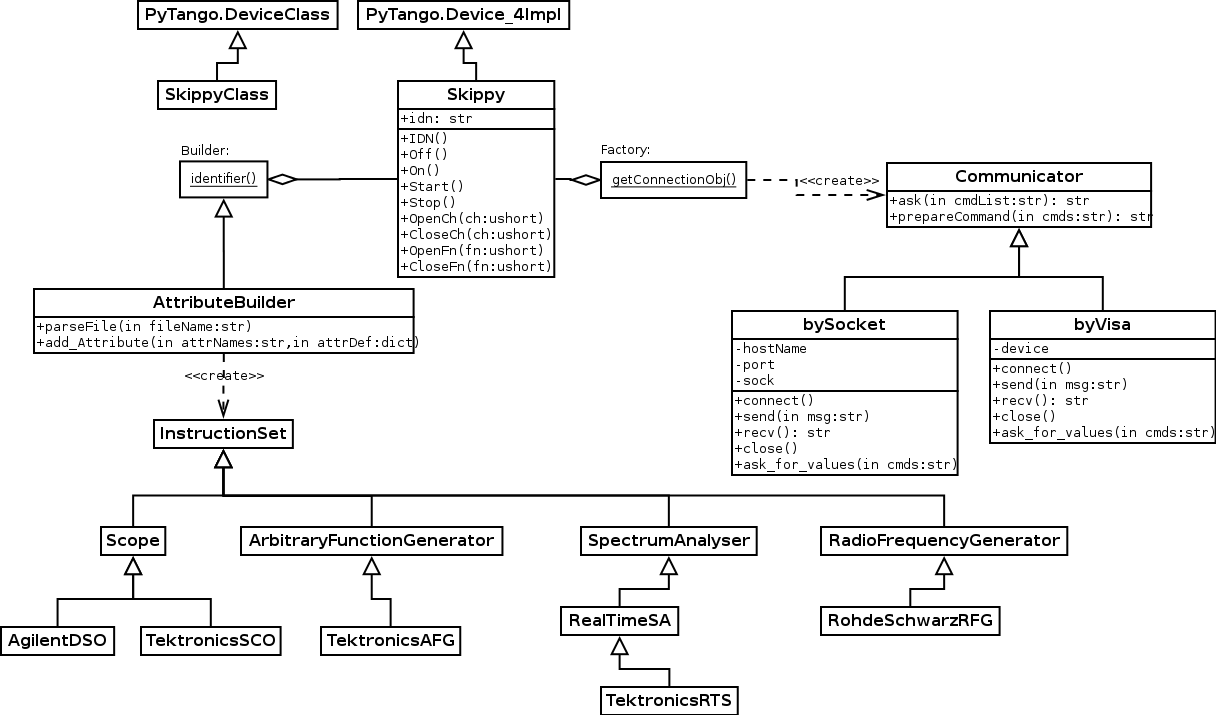
\includegraphics[width=\textwidth]{ClassDiagram.png}
         \caption{Class diagram of the Skippy device.} \label{fig:classDiagram}
    }
\end{figure}

\subsection{Device features}

\begin{itemize}
    \item Device is capable to dynamically build attributes based on the instrument identification (described in the the particular instruction set).
    \begin{itemize}
        \item Supported Scalar and Spectrum (1 dimension arrays) attribute definition. Image (2 dimension arrays) are not currently developed, neither in the schedule because they are not needed by any of the current supported instruments. Although the device is prepared to sopport them if need be. (Perhaps the frequencies spectra in SpectrumAnalyser).
        \item \todo{Memorized dynamic attributes.}
        \item \todo{Reconnect after network cut (or PyVisa)}
    \end{itemize}
    \item Multiple request of data to the instrument: As figure \ref{fig:groupedRequests} describes, when the device receives a request for reading to the instrument it can manage to cut those requests in subsets to avoid stress in the instrument. The communication itself supports a direct socket connection to the instrument and the use of the PyVisa device as a bridge in the communication.
\end{itemize}

\begin{figure}[h]
    \centering{
         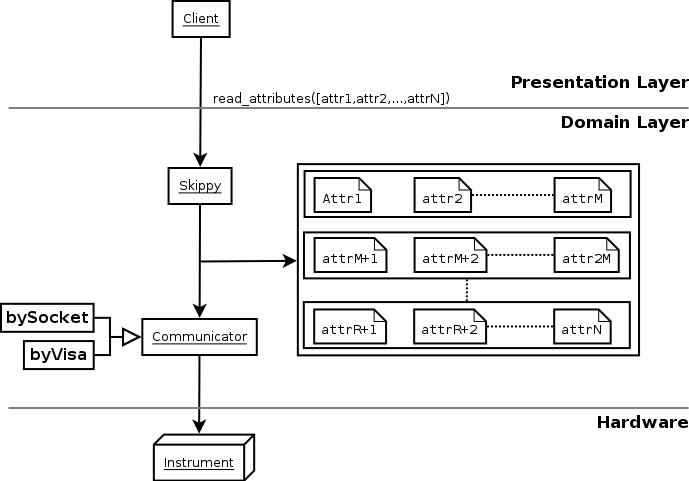
\includegraphics[width=0.75\textwidth]{groupedRequests.png}
         \caption{multiple request of readings to the instrument.} \label{fig:groupedRequests}
    }
\end{figure}

\begin{itemize}
    \item \todo{Write process to some attributes would require a smooth ramp. As an example, to change the frequency in the RFGenerator, the change would not be set directly (or the timing system will suffer). Then in the build process of an specific attribute with a certain flag of "movability" (name to be determined) two extra attributes, internals in the device, must be built also: a Step and a StepSpeed. On the write operation a thread should be launched and every "StepSpeed" seconds change the value by the content in "Step" in the direction to the final setpoint. This was already implemented in PyRfSignalGenerator Class.}
    \item \todo{Monitor attributes. Having a property with a list of attributes, if they exist in the instrument definition, configure them in events and do a separeted thread polling that will emit events on this attributes. This feature is different that setting up a "polling" from tango to the attribute because this fails to use the multiple reading.}
    \begin{itemize}
        \item Perhaps in the definition of the attributes to be monitored, extra information can be added to allow different polling periods each.
        \item Also a command way feature is required to add and remove elements from this monitoring list.
    \end{itemize}
    \item \todo{Once this monitoring feature is available, other attributes not monitored that have reached some reading frequency, would be included in the monitoring loop (not emitting events) in order to reduce the load of the readings. The frequency reading should be monitored to notice when this has reduced over another threshold to avoid unnecessary readings.}
\end{itemize}


\end{document}
